\clearpage

\section{Supporting Information}

% \subsection{Table of contents and index}
%%%%%%%%%%%%%%%%%%%%%%%%%%%%%%%%%%%%%%%%%%%%%%%%%%%%%%%%%%%%%%%%%%%%%%%%%%%%%%%%
% The table of contents and index are quite important and should follow general compositional practices.
%%%%%%%%%%%%%%%%%%%%%%%%%%%%%%%%%%%%%%%%%%%%%%%%%%%%%%%%%%%%%%%%%%%%%%%%%%%%%%%%

\subsection{Appendixes}

%%%%%%%%%%%%%%%%%%%%%%%%%%%%%%%%%%%%%%%%%%%%%%%%%%%%%%%%%%%%%%%%%%%%%%%%%%%%%%%%
% The appendixes are not always considered part of the actual SRS and are not always necessary.
% They may include
% 
% 1. Sample input/output formats, descriptions of cost analysis studies, or results of user surveys;
% 
% 2. Supporting or background information that can help the readers of the SRS;
% 
% 3. A description of the problems to be solved by the software;
% 
% 4. Special packaging instructions for the code and the media to meet security, export, initial loading, or other requirements.
% 
% When appendixes are included, the SRS should explicitly state whether or not the appendixes are to be considered part of the requirements.
%%%%%%%%%%%%%%%%%%%%%%%%%%%%%%%%%%%%%%%%%%%%%%%%%%%%%%%%%%%%%%%%%%%%%%%%%%%%%%%%

\begin{figure}[hp]
  \centering
  \captionsetup{justification=centering,margin=2cm}
  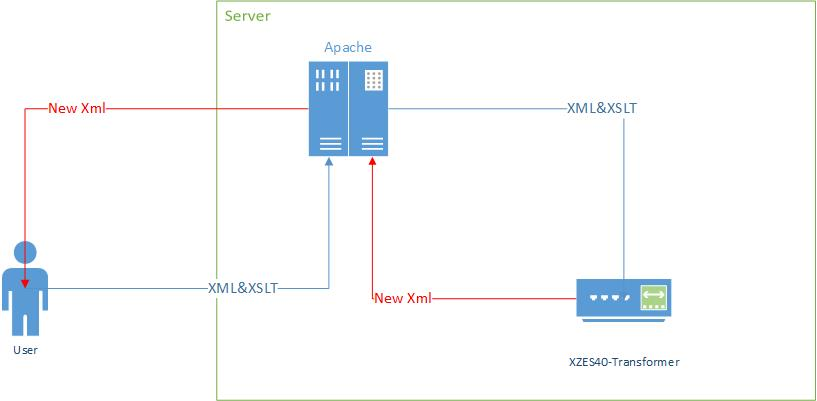
\includegraphics[width=0.5\textwidth]{figures/document-flow-digram}
  \caption{
    Diagram of dataflow.
    Documents are sent to the application through the Apache gateway interface.
    Once processed documents are returned to the user through the gateway interface again.
  }
\end{figure}
        
\begin{figure}[hp]
  \centering
  \captionsetup{justification=centering,margin=2cm}
  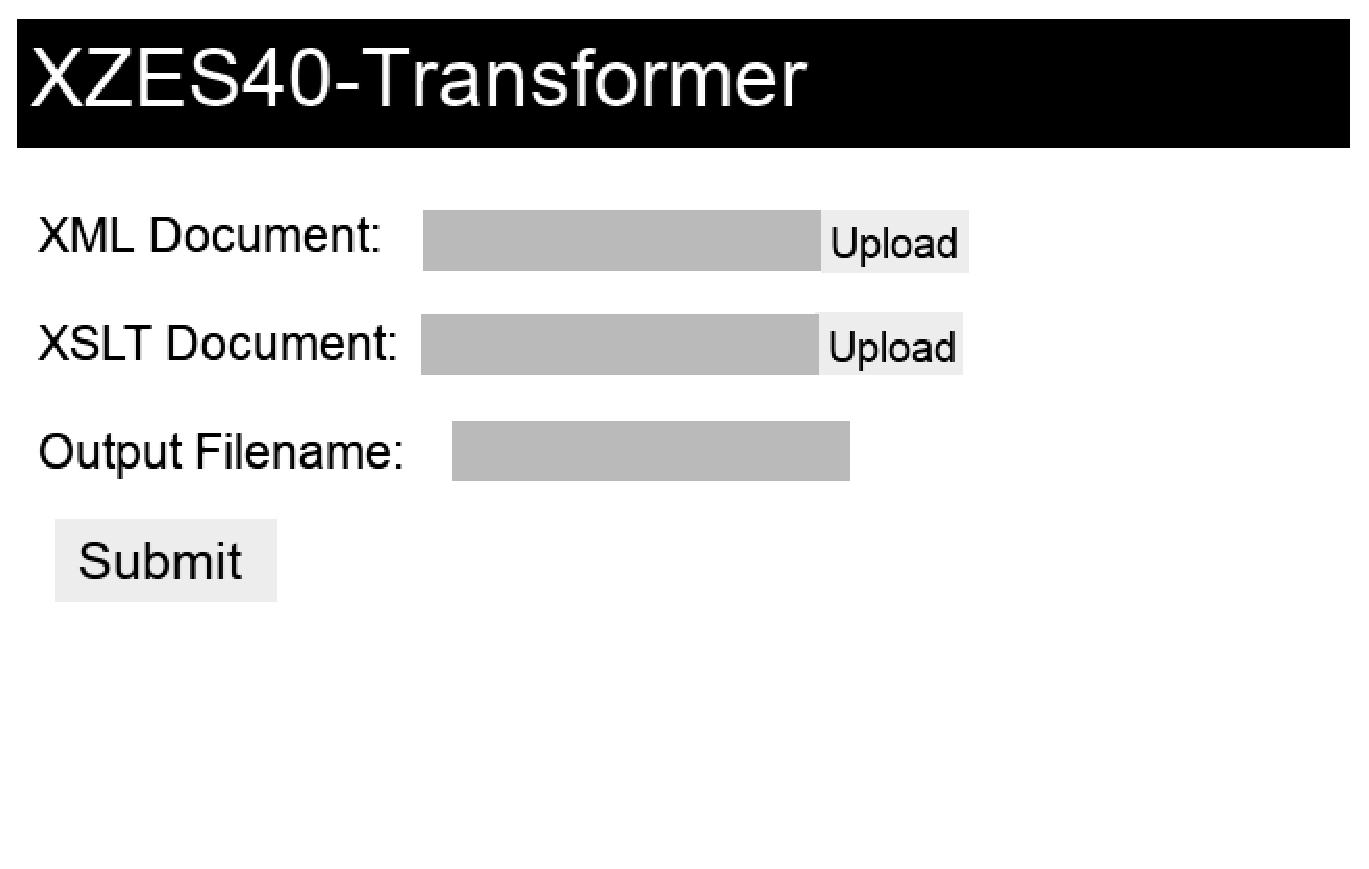
\includegraphics[width=0.5\textwidth]{figures/website-raw}
  \caption{
    Prototype of the Web Interface.
    Demonstrates the simplicity of the interface and required form fields.
  }
\end{figure}

\begin{figure}[hp]
  \centering
  \captionsetup{justification=centering,margin=2cm}
  \begin{lstlisting}
Normal usage:
$ xzes40cli --xml-file='./my-file.xml' --xslt-file='./my-other-file.xslt' --server='http://example.com/xzes40-transformer' --output-file='./newfile.xml' --port='8001'
Sending XML and XSLT files to http:/example.com:8001/xzes40-transformer
Transformation complete. Downloading response file to newfile.xml

Sending a bad file:
$ xzes40cli --xml-file='./badfile.jpg' --xslt-file='./badfile.txt' --server='http://example.com/xzes40-transformer'
Sending XML and XSLT files to http:/example.com:80/xzes40-transformer
ERROR: Server was unable to transform the requested files.

Using inadequate parameters
$ xzes40cli
Please provide an xml file (--xml-file), xslt file (--xslt-file) and a host (--server).
  \end{lstlisting}
  \caption{Example use-cases of CLI interface.}
\end{figure}

\begin{figure}[hp]
  \centering
  \captionsetup{justification=centering,margin=2cm}
  \begin{PstGanttChart}[yunit=1,
                        xunit=1,
                        ChartUnitIntervalName=W,
                        ChartUnitBasicIntervalName=W,
                        TaskUnitIntervalValue=10,
                        TaskUnitType=W,
                        ChartStartInterval=1,
                        ChartShowIntervals]{20}{19}
   \psset{gradangle=180}
   \PstGanttTask[TaskStyle=Important,TaskInsideLabel={Alpha}]{0}{6}
   \PstGanttTask[TaskInsideLabel={Benchmark Data Collection}]{0}{3}
   \PstGanttTask[TaskInsideLabel={Core Functionality}]{0}{11}
   \PstGanttTask[TaskInsideLabel={Basic Transformation}]{0}{3}
   \PstGanttTask[TaskInsideLabel={Caching}]{3}{7}
   \PstGanttTask[TaskInsideLabel={Parallel Computation}]{3}{7}
   \PstGanttTask[TaskInsideLabel={Demo}]{5}{1}
   \PstGanttTask[TaskStyle=Important,TaskInsideLabel={Beta}]{6}{5}
   \PstGanttTask[TaskInsideLabel={CGI Script}]{7}{1}
   \PstGanttTask[TaskInsideLabel={Web Interface}]{8}{2}
   \PstGanttTask[TaskInsideLabel={Debian Package}]{9}{2}
   \PstGanttTask[TaskInsideLabel={Demo}]{10}{1}
   \PstGanttTask[TaskStyle=Important,TaskInsideLabel={Release}]{12}{7}
   \PstGanttTask[TaskInsideLabel={CLI Interface}]{12}{2}
   \PstGanttTask[TaskInsideLabel={RedHat Package}]{12}{6}
   \PstGanttTask[TaskInsideLabel={BSD Package}]{12}{6}
   \PstGanttTask[TaskInsideLabel={Windows Package}]{12}{6}
   \PstGanttTask[TaskInsideLabel={Demo}]{17}{2}
   \PstGanttTask[TaskStyle=NotImportant]{11}{1}
  \end{PstGanttChart}
  \caption{Development Gantt Chart Timeline.}
\end{figure}
